\chapter{The Study of H$\alpha$ Emission Spectra}

\section{Context and Relevance}
P Cygni and inverse P Cygni spectra are sub classes of H$\alpha$ emission spectra \cite{zhang2021catalog}. The identification of H$\alpha$ emission spectra in large scale spectroscopic surveys is an active area of research.\cite{zhang2021catalog,vcotar2021galah,traven2015gaia}. Thus the identification of H$\alpha$ emission spectra can serve as a useful precursor to identifying P Cygni and inverse P Cygni spectra. This approach can be extremely beneficial in reducing the search space as well the feature space that may serve as input data to a detection and identification pipeline that is tuned to identify P Cygni and inverse P Cygni spectra. 

This chapter presents a brief summary of recent methods employed to identify H$\alpha$ emission spectra, in both smaller scale observations as well as large scale surveys. These are placed in the context of their importance in the identification of P Cygni and inverse P Cygni spectra.

\section{A Historical Perspective}
An atlas of high resolution line profiles with H$\alpha$ emissions was provided by Vam Winckel at al. in 1993\cite{van1993atlas}. The authors provide a classification scheme for H$\alpha$ spectra based on their morphology. The spectra were identified and classified using manual methods. Direct visual inspection and measurement of the width and shape of the line profile was used to classify these spectra. In particular, wind velocity dispersions outside the primary disk of the star were used to determine the membership of candidates in each class.
A few of the classes identified by the authors include, subtype S1, narrow emission with no prominent absorption; subtype S2 which shows a clear absorption feature superimposed on a broad emission feature; and subtype S3 which shows a strong absorption feature which reaches at least the continuum level. The authors note that the radial velocities of the 59 emission lines considered were generally redshifted. It is noteworthy that this study used wind velocity dispersions to classify the spectral types. For example, S3 showed the smallest wind velocity dispersion, thus demonstrating a relationship between the morphology of the spectra and the physical processes that generate them.

\begin{figure}[h]
\centering
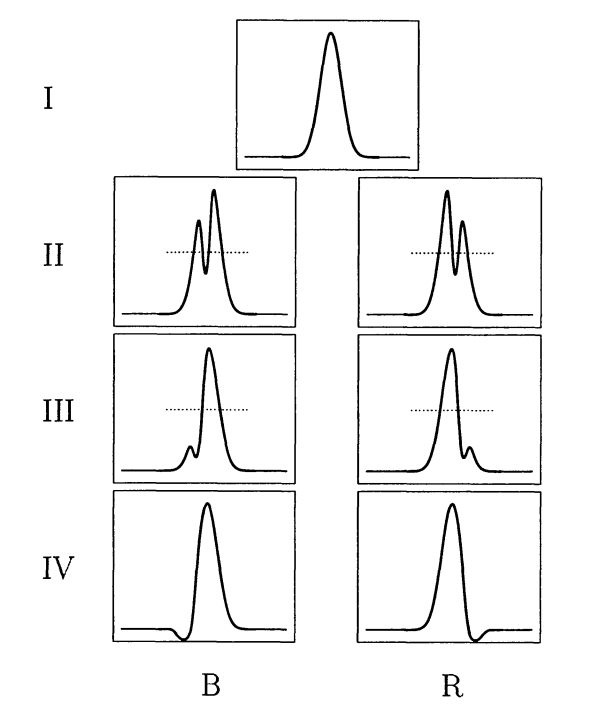
\includegraphics[scale=0.75]{figures/reipurth classes.png}
\caption{The morphology based classification scheme proposed by Reipurth et al. Depending on the location of the primary peak in relation to the secondary peak, the letters B and R are appended to the Roman numerals. They stand for blue-shifted and red-shifted respectively.}
\end{figure}

Published in 1996, Reipurth et al. studied the H$\alpha$ profiles of pre-main sequence stars using manual methods. In addition to identifying T Tauri stars and Ae/Be stars using high resolution spectra (R~50,000), the study focused on the morphological properties of P Cygni stars as well as the physical processes that generate them. The study notes the discovery of complex morphological profiles among the T Tauri, Ae/Be and P Cygni stars. 

The authors proposed a two dimensional classification scheme based on the relative height of a secondary peak compared to the primary peak, as well as whether the absorption line is blue or red shifted. The authors note the classification of 25\% symmetric profiles, 49\% blue shifted absorption profiles and 5\% P-Cygni profiles amongst the observed spectra. Of the spectra, 21\% fall into the redshifted absorption category. In addition to this morphological classification, the authors also presented wind velocities of the samples with some stars recording extremely high velocities of ~ 900km/s \cite{reipurth1996halpha}. 

The classification of P Cygni stars in this paper follow the scheme proposed by Beals in 1953\cite{1953PDAO....9....1B}. The authors have also presented a discussion comparing observed data to models in literature, particularly models that constrain mass, radii and photospheric temperatures. No specific model details for P Cygni stars were provided. Further catalogues of H$\alpha$ emission stars have been provided by Kohoutek and Wehmeyer (1997 and 1999). These catalogues contain 98 identified emission-line stars in the Northern Milky Way. These catalogues do not specifically identify P Cygni stars or inverse P Cygni stars \cite{kohoutek1999catalogue}.

The study of open clusters such as NGC 6611 and others have pushed our understanding of H$\alpha$ emission stars \cite{bonito2013spectroscopic,traven2015gaia}. Bonito et al. in particular note that for stars surrounded by active disks the morphology of the emission lines could fall into categories such as symmetric with broad wings, asymmetric and in extreme cases, P Cygni and inverse P Cygni. The authors have used the classification scheme proposed by Reipurth et al and have adhered to the type I - IV scheme with B and R suffixes to denote blue shifted and red shifted emission lines respectively. 

Traven et al. presented a catalogue of H$\alpha$ emission stars in the Gaia-ESO survey. This survey is biased towards young open clusters and consequently, the authors note a relatively large proportion of H$\alpha$ emission candidates that were identified in this work. The authors note the identification of 3765 emission stars from a sample of 22035 spectra from the Gaia-ESO survey. This work is notable as it uses a combination of empirical rules and automated techniques like spectral fitting to sort the H$\alpha$ emission spectra into eight distinct morphological categories: single–component emission, emission blend, sharp emission peaks, double emission, P-Cygni, inverted P-Cygni, self–absorption, and emission in absorption \cite{traven2015gaia}. The Gaia-ESO survey had conducted repeat observations of about half the identified H$\alpha$ emission stars. Thus the authors were able to comment on the temporal variability of these stars. The conclusion was that while some morphological categories exhibited stability of their spectral profiles over time, P-Cygni and self-absorption profiles may not. Supplementary information of these candidates from SIMBAD, VizieR and ADS were also provided. In addition to this data, the authors have provided wind velocity estimates based on the automated curve fitting procedure. The authors note that the identification, classification and characterisation of emission stars can be valuable for automatic pipelines in large surveys (e.g. GALAH), where they can pinpoint outliers when calculating general stellar properties and abundances. Additionally, they note that the identified stars can be used in studies of star formation processes, interacting binaries and related fields of stellar physics. 

The historical review allow us to draw a number of conclusions:

\begin{enumerate}
\item These methods relied exclusively on visual inspection of spectra and manual methods to identify H$\alpha$ candidates. While this may have been a suitable approach in the past, it is extremely challenging to extend and scale these methods to datasets generated by million star all sky surveys in the modern era. Thus this project does not consider these manual methods for the detection of H$\alpha$ candidates as well as P Cygni and inverse P Cygni spectra. 

\item Morphology based classification approaches as demonstrated by Reipurth et al. and even Beals are significantly important. It was demonstrated in Chapter 1 that the variety of spectral morphologies are hypothesised to be generated due to distinct physical phenomena linked to the stellar disk and the gas that surrounds it. This research leans into this approach and relies on morphological similarities and dissimilarities as a basis for spectral classification.

\item Finally, these studies have identified P Cygni and inverse P Cygni (among other classes of spectra) as forming a subset of H$\alpha$ emission spectra. This project exploits this fact to it's logical conclusion i.e. the probability of automated detection of P Cygni and inverse P Cygni spectra can be increased if the search space and feature space of the raw data can be reduced from the complete DR3 catalog, to a much narrower subset of H$\alpha$ emission candidates identified in DR3.
\end{enumerate}

\section{Recent Developments}

The increase in data availability via large scale spectroscopic surveys has necessitated and demanded the use of semi automated and fully automated methods. Morphology based classification has been adopted by many researchers in the field and augmented by statistical methods and machine learning. In general, machine learning approaches can fall into two categories; supervised and unsupervised learning. The former relies on the availability of a suitably robust set of training examples while the latter attempts to generalise and learn from unlabelled data \cite{hastie2009elements}. A full discussion and review of machine learning methods is beyond the scope of this thesis. Techniques and methods that are relevant to this research are presented in text. Chapter 4 in particular will present a more detailed discussion on methods that are relevant to the present thesis. This section reviews four recent approaches that rely on machine learning to detect and characterise H$\alpha$ candidates, their strengths and limitations.

\subsection{The Use K-means Clustering for APOGEE Spectra}

K-means clustering is a well known unsupervised clustering algorithm.The goal of this algorithm is to partition a set of observations into a predefined set of clusters. Each observation would belong to a cluster with the nearest mean which serves as the centroid or prototype of the cluster \cite{macqueen1967some}. Formally, given a set of $n$ observations such as \(x_1,x_2,...,x_n\) where each observation is a $d$ dimensional vector, the algorithm will partition the $n$ observations into $k$ sets $S=\{S_1,S_2,...,S_k\}$ such that within cluster variance is minimised. This objective can be represented as:

\begin{equation}
{\underset {\mathbf {S} }{\operatorname {arg\,min} }}\sum _{i=1}^{k}\sum _{\mathbf {x} \in S_{i}}\left\|\mathbf {x} -{\boldsymbol {\mu }}_{i}\right\|^{2}={\underset {\mathbf {S} }{\operatorname {arg\,min} }}\sum _{i=1}^{k}|S_{i}|\operatorname {Var} S_{i}
\end{equation}

where $\mu_i$ is the mean of the points in $S_i$. 

Using the identity:

\begin{equation}
    |S_{i}|\sum _{\mathbf {x} \in S_{i}}\left\|\mathbf {x} -{\boldsymbol {\mu }}_{i}\right\|^{2}=\sum _{\mathbf {x} \neq \mathbf {y} \in S_{i}}\left\|\mathbf {x} -\mathbf {y} \right\|^{2}
\end{equation}

It can be shown that this is equivalent to minimising the pairwise squared deviations of points belonging to the same cluster:

\begin{equation}
{\underset {\mathbf {S} }{\operatorname {arg\,min} }}\sum _{i=1}^{k}\,{\frac {1}{|S_{i}|}}\,\sum _{\mathbf {x} ,\mathbf {y} \in S_{i}}\left\|\mathbf {x} -\mathbf {y} \right\|^{2}
\end{equation}

APOGEE which is part of the Sloan Digital Sky Survey (SDSS) is a high resolution spectroscopic survey (R$\approx$ 22,500) \cite{eisenstein2001spectroscopic,blanton2017sloan}. In the absence of labelled training samples in the APOGEE survey Garcia-Dias et al. used k-means to cluster similar spectra into distinct groups \cite{garcia2018machine}. Each spectrum produced by APOGEE was treated as a $d$ dimensional vector. The number of observations $n$ was the number of spectra generated by APOGEE which was approximately 150,000. $k$ was set to 50. The authors note that they were able to separate dwarfs, sub-giants, RC and RGB stars. The authors note that the approach is sensitive to initialisation and thus sensitive to the number of clusters $k$. One major limitation of this approach is that a discrete classification in the flux space does not result in a neat organisation in the parameters' space. The other limitation being the use of manual sorting of clusters that reduced the number of clusters from 50 to 9. This implies that certain spectra were incorrectly clustered by the k-means algorithm. The authors were unable to cluster H$\alpha$ emission spectra using this method. The primary conclusion that can be drawn from this work is that k-means clustering may perform poorly if it is used to cluster and ultimately classify morphologically similar spectra such as P Cygni and inverse P Cygni. A methodology that relates the flux space, and consequently the morphology of the spectrum, to a parameter space may perform better than k-means. 

\subsection{Automated and Manual Methods for LAMOST Spectra}

The LAMOST survey is a low resolution spectroscopic survey with 10 million Milky Way stars as potential survey candidates. Zhang et al. were able to use a training and test set (labelled spectra) comprising 5,915 samples for spectral classification. This training set was based on data released by Hou et al. \cite{hou2016catalog} who developed the datsset by visually examining LAMOST spectra. The existence of labelled data including seven P Cygni and inverse P Cygni spectra identified by Hou et al. was exploited for supervised machine learning algorithms. As such, 10 different supervised learning methods were then applied to this dataset including including KNN (K-Nearest Neighbor), RF (Random Forest), AdaBoost, Naive Bayes (MultinomialNB, GaussianNB, BernoulliNB), logistic regression, SVM (Support Vector Machine) and Artificial Neural Network (Single-hidden Layer, Three-hidden Layer) \cite{zhang2021catalog}. A comparison of the performance of these methods were not provided by the author. However they note that the k-nearest neighbour and random forest methods outperformed all other methods. A detailed discussion of these methods is omitted from this thesis as it would be beyond the scope of this project. These two supervised machine learning models were then applied to 498,588 spectra resulting in 56,574 potential H$\alpha$ emission candidates. These candidates were then visually inspected with a final candidate list of 30,048 H$\alpha$ emission spectra. A significant drawback of this approach is the reliance on manual visual inspection of spectra in building the training set as well as during classification of the identified potential H$\alpha$ emission spectra. A labelled training set with clearly identified P Cygni and inverse P Cygni spectra does not currently exist for GALAH DR3 and thus none of these methods can be extended to DR3. In the subsequent chapter, this author will demonstrate an automated method that generates such a dataset for GALAH DR3 which does not rely on manual visual inspection.





